\documentclass[]{article}
\usepackage{lmodern}
\usepackage{amssymb,amsmath}
\usepackage{ifxetex,ifluatex}
\usepackage{fixltx2e} % provides \textsubscript
\ifnum 0\ifxetex 1\fi\ifluatex 1\fi=0 % if pdftex
  \usepackage[T1]{fontenc}
  \usepackage[utf8]{inputenc}
\else % if luatex or xelatex
  \ifxetex
    \usepackage{mathspec}
  \else
    \usepackage{fontspec}
  \fi
  \defaultfontfeatures{Ligatures=TeX,Scale=MatchLowercase}
\fi
% use upquote if available, for straight quotes in verbatim environments
\IfFileExists{upquote.sty}{\usepackage{upquote}}{}
% use microtype if available
\IfFileExists{microtype.sty}{%
\usepackage{microtype}
\UseMicrotypeSet[protrusion]{basicmath} % disable protrusion for tt fonts
}{}
\usepackage[margin=1in]{geometry}
\usepackage{hyperref}
\hypersetup{unicode=true,
            pdftitle={Econometria - Series Temporais},
            pdfborder={0 0 0},
            breaklinks=true}
\urlstyle{same}  % don't use monospace font for urls
\usepackage{color}
\usepackage{fancyvrb}
\newcommand{\VerbBar}{|}
\newcommand{\VERB}{\Verb[commandchars=\\\{\}]}
\DefineVerbatimEnvironment{Highlighting}{Verbatim}{commandchars=\\\{\}}
% Add ',fontsize=\small' for more characters per line
\usepackage{framed}
\definecolor{shadecolor}{RGB}{248,248,248}
\newenvironment{Shaded}{\begin{snugshade}}{\end{snugshade}}
\newcommand{\AlertTok}[1]{\textcolor[rgb]{0.94,0.16,0.16}{#1}}
\newcommand{\AnnotationTok}[1]{\textcolor[rgb]{0.56,0.35,0.01}{\textbf{\textit{#1}}}}
\newcommand{\AttributeTok}[1]{\textcolor[rgb]{0.77,0.63,0.00}{#1}}
\newcommand{\BaseNTok}[1]{\textcolor[rgb]{0.00,0.00,0.81}{#1}}
\newcommand{\BuiltInTok}[1]{#1}
\newcommand{\CharTok}[1]{\textcolor[rgb]{0.31,0.60,0.02}{#1}}
\newcommand{\CommentTok}[1]{\textcolor[rgb]{0.56,0.35,0.01}{\textit{#1}}}
\newcommand{\CommentVarTok}[1]{\textcolor[rgb]{0.56,0.35,0.01}{\textbf{\textit{#1}}}}
\newcommand{\ConstantTok}[1]{\textcolor[rgb]{0.00,0.00,0.00}{#1}}
\newcommand{\ControlFlowTok}[1]{\textcolor[rgb]{0.13,0.29,0.53}{\textbf{#1}}}
\newcommand{\DataTypeTok}[1]{\textcolor[rgb]{0.13,0.29,0.53}{#1}}
\newcommand{\DecValTok}[1]{\textcolor[rgb]{0.00,0.00,0.81}{#1}}
\newcommand{\DocumentationTok}[1]{\textcolor[rgb]{0.56,0.35,0.01}{\textbf{\textit{#1}}}}
\newcommand{\ErrorTok}[1]{\textcolor[rgb]{0.64,0.00,0.00}{\textbf{#1}}}
\newcommand{\ExtensionTok}[1]{#1}
\newcommand{\FloatTok}[1]{\textcolor[rgb]{0.00,0.00,0.81}{#1}}
\newcommand{\FunctionTok}[1]{\textcolor[rgb]{0.00,0.00,0.00}{#1}}
\newcommand{\ImportTok}[1]{#1}
\newcommand{\InformationTok}[1]{\textcolor[rgb]{0.56,0.35,0.01}{\textbf{\textit{#1}}}}
\newcommand{\KeywordTok}[1]{\textcolor[rgb]{0.13,0.29,0.53}{\textbf{#1}}}
\newcommand{\NormalTok}[1]{#1}
\newcommand{\OperatorTok}[1]{\textcolor[rgb]{0.81,0.36,0.00}{\textbf{#1}}}
\newcommand{\OtherTok}[1]{\textcolor[rgb]{0.56,0.35,0.01}{#1}}
\newcommand{\PreprocessorTok}[1]{\textcolor[rgb]{0.56,0.35,0.01}{\textit{#1}}}
\newcommand{\RegionMarkerTok}[1]{#1}
\newcommand{\SpecialCharTok}[1]{\textcolor[rgb]{0.00,0.00,0.00}{#1}}
\newcommand{\SpecialStringTok}[1]{\textcolor[rgb]{0.31,0.60,0.02}{#1}}
\newcommand{\StringTok}[1]{\textcolor[rgb]{0.31,0.60,0.02}{#1}}
\newcommand{\VariableTok}[1]{\textcolor[rgb]{0.00,0.00,0.00}{#1}}
\newcommand{\VerbatimStringTok}[1]{\textcolor[rgb]{0.31,0.60,0.02}{#1}}
\newcommand{\WarningTok}[1]{\textcolor[rgb]{0.56,0.35,0.01}{\textbf{\textit{#1}}}}
\usepackage{graphicx,grffile}
\makeatletter
\def\maxwidth{\ifdim\Gin@nat@width>\linewidth\linewidth\else\Gin@nat@width\fi}
\def\maxheight{\ifdim\Gin@nat@height>\textheight\textheight\else\Gin@nat@height\fi}
\makeatother
% Scale images if necessary, so that they will not overflow the page
% margins by default, and it is still possible to overwrite the defaults
% using explicit options in \includegraphics[width, height, ...]{}
\setkeys{Gin}{width=\maxwidth,height=\maxheight,keepaspectratio}
\IfFileExists{parskip.sty}{%
\usepackage{parskip}
}{% else
\setlength{\parindent}{0pt}
\setlength{\parskip}{6pt plus 2pt minus 1pt}
}
\setlength{\emergencystretch}{3em}  % prevent overfull lines
\providecommand{\tightlist}{%
  \setlength{\itemsep}{0pt}\setlength{\parskip}{0pt}}
\setcounter{secnumdepth}{0}
% Redefines (sub)paragraphs to behave more like sections
\ifx\paragraph\undefined\else
\let\oldparagraph\paragraph
\renewcommand{\paragraph}[1]{\oldparagraph{#1}\mbox{}}
\fi
\ifx\subparagraph\undefined\else
\let\oldsubparagraph\subparagraph
\renewcommand{\subparagraph}[1]{\oldsubparagraph{#1}\mbox{}}
\fi

%%% Use protect on footnotes to avoid problems with footnotes in titles
\let\rmarkdownfootnote\footnote%
\def\footnote{\protect\rmarkdownfootnote}

%%% Change title format to be more compact
\usepackage{titling}

% Create subtitle command for use in maketitle
\providecommand{\subtitle}[1]{
  \posttitle{
    \begin{center}\large#1\end{center}
    }
}

\setlength{\droptitle}{-2em}

  \title{Econometria - Series Temporais}
    \pretitle{\vspace{\droptitle}\centering\huge}
  \posttitle{\par}
    \author{}
    \preauthor{}\postauthor{}
    \date{}
    \predate{}\postdate{}
  

\begin{document}
\maketitle

Ativando os pacotes

Importando o banco de dados \#exemplo bd, criado de forma aleatoria

\begin{Shaded}
\begin{Highlighting}[]
\NormalTok{dados<-}\StringTok{ }\KeywordTok{read.delim}\NormalTok{(}\StringTok{"D:/Google Drive/2 - Ufpb/P5/Econometria/Series/Dados/dadosseriestemporais.txt"}\NormalTok{)}
\NormalTok{dados}
\end{Highlighting}
\end{Shaded}

\begin{verbatim}
##         ano        DE     FP    IC    SC   TD
## 1   1995.01  46331.44  78.13 124.4 48.92  7.9
## 2   1995.02  46818.79  77.68 123.9 46.83  8.9
## 3   1995.03  48113.47  81.66 114.1 65.01  9.2
## 4   1995.04  50658.81  83.38 106.2 64.88  9.4
## 5   1995.05  53979.63  87.56 105.3 64.74  9.2
## 6   1995.06  56569.92  88.76 102.2 60.84  9.1
## 7   1995.07  58557.33  89.14  98.0 60.53  9.1
## 8   1995.08  59466.12  89.20  97.1 57.17  8.8
## 9   1995.09  59253.58  86.66  97.5 48.06  9.0
## 10  1995.10  59891.43  90.13  97.4 44.11  9.0
## 11  1995.11  60450.73 102.35  97.4 40.52  9.1
## 12  1995.12  64266.65 124.97  98.0 38.92  8.7
## 13  1996.01  64902.72  96.41 101.4 35.70  8.5
## 14  1996.02  65233.10  95.03 104.0 32.17  9.1
## 15  1996.03  65267.82  93.05 108.2 30.16 10.1
## 16  1996.04  65114.54  91.85 107.7 27.84 11.0
## 17  1996.05  64692.97  93.87 104.6 27.01 10.8
## 18  1996.06  64510.54  94.97 105.3 26.49 10.7
## 19  1996.07  64278.98  97.10 105.6 25.76 10.3
## 20  1996.08  64236.00  97.83 107.2 26.35 10.3
## 21  1996.09  64726.91  97.61 106.8 25.40  9.9
## 22  1996.10  65754.07  97.14 109.4 24.73  9.7
## 23  1996.11  67558.05 108.59 111.7 23.93  9.6
## 24  1996.12  72652.00 138.35 112.2 23.94  9.2
## 25  1997.01  77130.33 101.62 114.3 22.88  8.9
## 26  1997.02  78711.82  97.11 112.8 22.02  9.1
## 27  1997.03  80034.28  98.39 115.9 21.58  9.9
## 28  1997.04  80883.31  98.20 117.0 21.84 10.7
## 29  1997.05  81791.65  98.25 109.4 20.76 10.7
## 30  1997.06  82927.44  98.67 106.1 21.08 10.5
## 31  1997.07  83626.27 100.64 108.4 21.04 10.2
## 32  1997.08  85063.78  98.10 105.7 20.78 10.2
## 33  1997.09  86591.73  97.79  98.7 20.84 10.5
## 34  1997.10  88145.78  97.99  96.9 22.03 10.5
## 35  1997.11  93941.90 110.44  98.0 43.30 10.5
## 36  1997.12  98211.26 136.19  93.5 42.12 10.2
## 37  1998.01 100628.94  99.99  94.5 37.19 10.3
## 38  1998.02  98600.98  95.68 103.2 29.85 11.1
## 39  1998.03  98108.16  94.76 100.5 29.85 12.0
## 40  1998.04  97850.78  93.11  91.0 22.52 12.5
## 41  1998.05  98234.21  95.42  87.7 21.41 12.4
## 42  1998.06  99703.66  94.21  93.8 21.02 12.3
## 43  1998.07 101146.46  93.65 102.7 22.47 12.1
## 44  1998.08 102317.11  91.50 109.4 19.23 12.0
## 45  1998.09 104162.81  89.41 112.4 34.29 11.7
## 46  1998.10 105773.76  90.39 113.3 41.60 11.6
## 47  1998.11 107168.49 100.64 106.9 36.58 11.3
## 48  1998.12 108442.38 122.15  92.7 32.95 10.8
## 49  1999.01 109360.15  89.15  94.2 29.50 10.7
## 50  1999.02 111432.30  84.90  89.9 32.59 11.6
## 51  1999.03 112363.68  86.10  75.7 48.23 12.9
## 52  1999.04 112524.50  85.04  75.9 32.18 13.4
## 53  1999.05 113364.45  86.34  77.3 27.11 12.9
## 54  1999.06 112787.04  86.06  91.5 22.01 12.5
## 55  1999.07 112300.92  86.51  99.1 21.83 12.6
## 56  1999.08 111709.81  85.77  98.2 20.53 12.4
## 57  1999.09 110964.42  85.78  99.0 19.38 12.2
## 58  1999.10 110498.34  87.34  95.5 17.93 11.6
## 59  1999.11 110695.59  99.49  93.9 17.97 11.4
## 60  1999.12 111406.67 123.45  94.6 20.98 10.5
## 61  2000.01 112685.74  94.76 100.9 18.94 10.6
## 62  2000.02 111879.54  92.27 107.3 18.87 10.5
## 63  2000.03 111304.74  91.54 100.1 18.85 11.3
## 64  2000.04 110935.78  90.22  93.9 16.71 11.8
## 65  2000.05 110441.69  91.48  89.4 19.48 11.8
## 66  2000.06 111044.99  91.89  94.5 18.04 11.7
## 67  2000.07 111006.66  93.66  98.3 16.85 11.6
## 68  2000.08 110716.14  91.95  91.2 18.23 11.2
## 69  2000.09 109494.43  90.94  92.0 15.71 11.0
## 70  2000.10 108731.59  93.37  98.5 16.60 10.4
## 71  2000.11 109260.19 105.32  99.4 15.66 10.3
## 72  2000.12 111936.10  91.87 100.8 15.36 10.0
## 73  2001.01 112272.26 100.00 111.3 16.28 10.1
## 74  2001.02 112831.87  98.43 113.5 12.89 10.7
## 75  2001.03 112398.66 109.13 108.6 16.18 11.2
## 76  2001.04 112749.02 116.22 105.2 15.20 11.5
## 77  2001.05 113891.73 109.82 102.4 17.27 11.0
## 78  2001.06 114874.37 108.84  79.4 16.40 10.7
## 79  2001.07 115508.72 109.21  87.2 19.53 10.9
## 80  2001.08 116060.60  85.80  86.4 20.98 11.3
## 81  2001.09 116737.77  98.42  90.7 17.10 11.5
## 82  2001.10 116399.42  89.49  80.7 20.06 11.9
## 83  2001.11 117676.13  99.62  78.3 18.06 11.7
## 84  2001.12 120030.42 129.37  86.3 18.07 11.6
## 85  2002.01 120034.06 114.40  87.0 20.04 11.3
## 86  2002.02 120495.52 104.33  90.7 16.05 12.0
## 87  2002.03 120786.60 133.33  91.3 17.76 12.8
## 88  2002.04 120419.32 140.31  96.0 19.33 13.3
## 89  2002.05 120908.90 127.01  96.2 18.37 12.8
## 90  2002.06 126974.87 127.69  84.4 17.17 12.0
## 91  2002.07 131996.17 122.69  93.8 20.06 11.5
## 92  2002.08 136876.68 101.35  89.8 18.76 11.8
## 93  2002.09 138721.22 117.96  99.2 17.89 12.2
## 94  2002.10 139529.47 122.05  94.9 21.64 12.3
## 95  2002.11 140309.02 105.99  98.7 20.14 12.0
## 96  2002.12 140895.70 120.41 102.9 23.03 11.4
## 97  2003.01 141282.81 123.67 103.0 26.40 11.2
## 98  2003.02 140814.92 133.24 103.5 24.32 11.9
## 99  2003.03 139704.83 150.89 101.9 23.54 12.7
## 100 2003.04 138719.21 158.07 107.7 24.92 13.6
## 101 2003.05 138432.05 144.76 112.0 26.31 13.4
## 102 2003.06 138247.44 146.91 116.8 24.70 13.2
## 103 2003.07 138812.24 131.20 111.5 28.09 12.7
## 104 2003.08 139451.14 104.52 109.4 23.50 12.9
## 105 2003.09 139195.38 133.82 106.4 22.12 13.2
## 106 2003.10 139129.36 118.14 104.7 21.59 13.2
## 107 2003.11 141200.60 120.50 108.7 17.37 12.6
## 108 2003.12 144118.43 135.72 115.3 17.78 12.0
## 109 2004.01 144683.60 140.33 124.2 16.32 11.9
## 110 2004.02 144902.04 133.84 123.4 13.82 12.6
## 111 2004.03 144291.74 203.70 113.3 17.86 13.3
## 112 2004.04 144734.92 200.19 108.0 15.14 13.2
## 113 2004.05 147287.54 181.74 124.2 15.77 12.3
## 114 2004.06 149287.47 194.60 117.1 15.80 11.8
## 115 2004.07 151502.62 184.17 118.5 16.58 11.7
## 116 2004.08 152155.18 177.55 120.7 16.68 11.7
## 117 2004.09 152920.90 182.48 128.4 16.09 11.4
## 118 2004.10 153680.11 146.46 141.9 15.57 10.8
## 119 2004.11 155244.31 153.20 145.0 16.09 10.4
## 120 2004.12 159588.79 180.94 140.4 19.32 10.0
## 121 2005.01 160218.69 162.33 145.0 17.93  9.9
## 122 2005.02 160232.29 147.92 146.5 15.64 10.4
## 123 2005.03 159708.51 206.63 145.0 19.96 10.9
## 124 2005.04 159438.24 217.23 141.8 18.32 11.1
## 125 2005.05 158834.89 207.72 133.6 19.61 11.0
## 126 2005.06 159920.73 218.92 132.7 20.78 11.0
## 127 2005.07 161792.50 205.04 133.2 19.72 10.8
## 128 2005.08 161674.96 191.45 124.9 21.82 10.6
## 129 2005.09 162195.29 194.85 109.2 19.61 10.4
## 130 2005.10 162628.36 183.98 107.7 18.26 10.6
## 131 2005.11 164240.58 161.03 117.2 17.89 10.2
## 132 2005.12 169322.67 249.09 130.2 19.19  9.7
## 133 2006.01 168740.22 169.70 131.5 18.57  9.5
## 134 2006.02 169964.48 171.42 138.0 14.64 10.2
## 135 2006.03 167242.33 203.62 137.8 18.47 10.9
## 136 2006.04 166661.12 240.09 132.4 13.73 11.2
## 137 2006.05 166049.30 191.14 138.2 16.51 11.3
## 138 2006.06 167620.32 207.15 134.4 15.18 11.3
## 139 2006.07 170109.60 207.24 134.2 14.98 11.3
## 140 2006.08 171003.43 179.66 128.2 16.16 10.7
## 141 2006.09 174233.25 196.67 131.4 13.45 10.3
## 142 2006.10 176209.35 145.95 132.3 13.95  9.6
## 143 2006.11 180118.52 157.65 134.6 12.96  9.1
## 144 2006.12 187864.03 168.26 127.5 12.52  9.0
## 145 2007.01 189734.96 134.61 133.9 13.80  9.0
## 146 2007.02 192044.83 154.41 134.4 10.99  9.7
## 147 2007.03 194873.23 170.74 127.9 13.38 10.4
## 148 2007.04 197639.65 185.45 128.0 11.95 10.9
## 149 2007.05 200246.41 194.50 126.5 13.06 10.6
## 150 2007.06 203955.12 209.24 129.8 11.43 10.3
## 151 2007.07 208214.26 182.30 130.1 12.32 10.5
## 152 2007.08 212971.47 161.37 130.3 12.58 10.4
## 153 2007.09 218432.22 175.34 131.8 10.10 10.5
## 154 2007.10 221168.74 127.57 133.3 11.74 10.0
## 155 2007.11 225354.95 177.32 136.3 10.62 10.0
## 156 2007.12 234671.90 177.59 139.9 10.62  9.3
## 157 2008.01 237490.43 206.24 142.6 11.74  9.3
## 158 2008.02 240438.78 194.59 146.9 10.06  9.1
## 159 2008.03 242582.02 183.04 147.7 10.62  9.6
## 160 2008.04 242699.02 191.40 148.6 11.37  9.8
## 161 2008.05 245170.73 191.35 147.4 11.04  9.8
## 162 2008.06 248087.17 207.95 142.6 12.09  9.7
## 163 2008.07 251930.71 191.00 131.2 13.62  9.6
## 164 2008.08 255225.91 178.19 137.1 12.92  9.4
## 165 2008.09 258397.67 182.31 141.3 14.07  9.3
## 166 2008.10 259940.52 135.49 140.5 15.06  8.5
## 167 2008.11 264128.86 158.49 133.9 12.95  8.6
## 168 2008.12 271156.74 193.53 128.7 14.36  8.3
## 169 2009.01 272499.57 176.17 125.2 13.32  9.2
## 170 2009.02 274852.75 218.35 134.1 10.76  9.8
## 171 2009.03 275496.47 181.89 130.9 12.29 10.8
## 172 2009.04 276043.85 204.07 126.3 10.55 10.9
## 173 2009.05 279463.48 214.00 129.0  9.65 10.8
## 174 2009.06 283038.10 218.60 140.0  9.54 10.3
## 175 2009.07 291041.25 216.45 145.0  9.90 10.5
## 176 2009.08 295603.41 189.22 145.6  8.65 10.1
## 177 2009.09 300498.35 209.01 148.8  8.65 10.1
## 178 2009.10 302983.25 162.13 157.2  8.65  9.9
## 179 2009.11 309223.99 178.04 155.8  8.21  9.4
## 180 2009.12 319631.93 203.48 156.6  9.12  8.5
## 181 2010.01 323908.66 188.85 160.5  8.21  8.0
## 182 2010.02 326604.36 210.78 161.4  7.31  8.5
## 183 2010.03 328636.03 204.89 159.9  9.51  9.6
## 184 2010.04 331852.08 215.87 154.7  8.34  9.8
## 185 2010.05 335901.45 218.60 155.8  9.38  9.7
## 186 2010.06 341889.87 231.48 160.6  9.90  9.5
## 187 2010.07 350691.95 224.49 157.2 10.82  9.4
## 188 2010.08 354495.99 221.02 164.5 11.22  9.3
## 189 2010.09 361242.17 202.28 162.6 10.69  8.7
## 190 2010.10 365719.67 163.69 155.4 10.16  8.4
## 191 2010.11 371209.62 179.90 160.1 10.16  8.1
## 192 2010.12 379604.27 200.02 164.3 11.45  7.4
## 193 2011.01 382043.99 182.74 160.8 10.85  8.0
## 194 2011.02 383334.10 217.67 164.2 10.61  8.1
## 195 2011.03 385733.26 187.75 160.3 11.62  9.0
## 196 2011.04 386122.94 212.34 159.4 10.56  8.8
## 197 2011.05 387046.56 217.92 153.0 12.52  8.5
## 198 2011.06 389558.70 225.61 153.8 12.10  8.7
## 199 2011.07 398005.68 229.46 152.9 12.25  8.8
## 200 2011.08 402719.24 231.55 152.7 13.68  9.0
## 201 2011.09 409310.51 208.51 154.1 11.91  8.5
## 202 2011.10 412717.60 176.73 151.9 11.11  7.9
## 203 2011.11 414983.46 188.02 155.4 10.83  7.5
## 204 2011.12 420872.65 250.40 158.2 11.45  6.9
## 205 2012.01 423261.83 200.01 158.3 11.23  7.6
## 206 2012.02 425054.07 232.69 170.2  9.36  8.4
## 207 2012.03 429860.85 221.77 164.4 10.31  9.1
## 208 2012.04 434077.04 222.80 165.0  8.88  9.1
## 209 2012.05 442527.44 237.71 163.1  9.31  8.8
## 210 2012.06 449801.59 234.92 162.4  7.98  9.0
## 211 2012.07 460241.95 240.25 160.6  8.47  9.1
## 212 2012.08 465932.01 219.67 156.3  8.63  9.4
## 213 2012.09 474052.53 223.85 158.3  6.66  9.1
## 214 2012.10 479470.97 177.87 161.4  7.59  8.5
## 215 2012.11 485716.89 209.88 159.7  6.79  7.9
## 216 2012.12 497139.07 271.25 161.8  6.81  7.6
## 217 2013.01 501669.86 249.95 160.6  7.46  7.8
## 218 2013.02 506417.66 235.02 165.8  6.08  8.2
## 219 2013.03 514654.97 229.65 160.0  6.80  8.8
## 220 2013.04 519548.89 248.45 155.6  7.62  9.1
## 221 2013.05 527860.46 246.30 146.0  7.42  9.0
## 222 2013.06 539315.24 256.53 145.0  7.51  9.1
## 223 2013.07 551158.75 275.61 136.7  9.04  9.0
## 224 2013.08 558449.22 254.85 133.0  8.86  8.6
## 225 2013.09 567882.04 311.47 136.7  8.90  8.1
## 226 2013.10 575369.02 195.33 139.2 10.17  7.7
## 227 2013.11 584781.09 233.07 138.0  8.98  7.5
## 228 2013.12 599825.99 259.37 136.6  9.90  7.5
## 229 2014.01 604824.60 314.94 131.7 10.68  7.8
## 230 2014.02 609877.47 254.36 136.4  9.90  8.7
## 231 2014.03 614875.53 470.16 125.8  9.59  9.4
## 232 2014.04 616830.71 255.57 120.3 10.33  9.6
## 233 2014.05 622339.69 256.64 109.5 10.90  9.5
## 234 2014.06 628926.42 265.61 107.4 10.35  9.4
## 235 2014.07 636446.77 288.60 109.6 12.00  9.4
## 236 2014.08 640564.03 274.37 110.5 10.90  9.2
## 237 2014.09 645474.10 307.97 118.9 11.45  8.7
## 238 2014.10 649650.21 208.17 115.8 12.02  8.1
## 239 2014.11 655806.26 237.50 116.0 10.59  7.9
## 240 2014.12 664847.30 236.60 113.0 12.17  8.0
## 241 2015.01 663517.45 258.53 112.7 11.82  7.9
## 242 2015.02 660210.26 255.43 112.9 10.33  8.7
## 243 2015.03 652549.19 382.40 106.9 13.22  9.4
## 244 2015.04 650444.73 295.58 101.6 12.04 10.2
## 245 2015.05 651079.30 263.25  91.8 12.49 10.7
## 246 2015.06 648879.27 267.99  90.6 13.58 11.1
## 247 2015.07 650714.09 297.03  84.6 15.09 11.4
## 248 2015.08 647539.58 263.54  84.7 14.15 11.5
## 249 2015.09 646378.45 281.29  85.5 14.15 11.8
## 250 2015.10 647197.56 218.67  88.8 14.15 11.9
## 251 2015.11 649996.77 227.97  85.6 13.43 11.7
## 252 2015.12 659005.51 237.94  87.2 14.87 11.5
## 253 2016.01 650996.72 263.54  89.0 13.43 11.8
## 254 2016.02 648289.78 281.29  95.2 12.72 12.3
## 255 2016.03 647003.07 218.67  89.3 14.87 13.4
## 256 2016.04 642773.09 227.97  87.7 13.43 14.2
## 257 2016.05 640246.59 237.94  90.9 14.15 15.0
## 258 2016.06 640680.04 263.54  98.1 14.87 14.7
## 259 2016.07 643807.20 281.29  97.7 14.15 14.2
## 260 2016.08 643658.87 218.67 100.1 15.60 13.9
## 261 2016.09 645433.35 227.97 107.0 14.15 14.4
## 262 2016.10 646800.71 237.94 106.0 13.34 14.3
## 263 2016.11 652682.55 263.54 110.3 13.20 14.0
## 264 2016.12 669286.30 281.29 110.7 14.34 13.5
## 265 2017.01 662201.48 218.67 102.3 13.84 14.1
## 266 2017.02 664105.90 227.97 113.8 10.89 14.8
## 267 2017.03 662919.50 229.65 109.4 13.38 15.2
## 268 2017.04 665181.33 255.57 109.0  9.86 15.5
## 269 2017.05 668998.34 256.64 103.5 11.71 15.9
## 270 2017.06 678744.38 265.61 100.1 10.15 15.6
## 271 2017.07 684707.83 288.60 104.8 10.01 15.1
## 272 2017.08 690409.72 281.29 101.5 10.06 14.5
## 273 2017.09 697406.90 218.67  99.7  7.94 14.5
## 274 2017.10 698581.33 227.97 102.8  8.01 14.8
## 275 2017.11 705588.13 237.94 104.0  7.04 14.1
## 276 2017.12 727981.35 263.54 109.5  6.66 12.9
## 277 2018.01 725734.25 281.29 117.0  7.24 13.2
## 278 2018.02 727848.59 218.67 120.6  5.73 13.6
## 279 2018.03 734825.27 281.29 115.6  6.58 14.5
## 280 2018.04 738795.11 218.67 109.9  6.40 14.4
## 281 2018.05 744039.51 227.97 113.5  6.40 14.2
## 282 2018.06 752524.35 229.65 104.0  6.40 14.1
## 283 2018.07 759125.38 227.97 103.5  6.71 14.6
## 284 2018.08 767980.28 237.94 104.4  7.03 14.4
## 285 2018.09 779246.72 263.54 106.8  5.77 13.9
## 286 2018.10 779696.01 281.29 107.9  6.71 13.1
## 287 2018.11 783382.48 293.53 114.5  6.09 12.4
## 288 2018.12 800889.43 296.36 127.8  6.09 12.5
\end{verbatim}

\begin{Shaded}
\begin{Highlighting}[]
\KeywordTok{class}\NormalTok{(dados)}
\end{Highlighting}
\end{Shaded}

\begin{verbatim}
## [1] "data.frame"
\end{verbatim}

\begin{Shaded}
\begin{Highlighting}[]
\NormalTok{dados}
\end{Highlighting}
\end{Shaded}

\begin{verbatim}
##         ano        DE     FP    IC    SC   TD
## 1   1995.01  46331.44  78.13 124.4 48.92  7.9
## 2   1995.02  46818.79  77.68 123.9 46.83  8.9
## 3   1995.03  48113.47  81.66 114.1 65.01  9.2
## 4   1995.04  50658.81  83.38 106.2 64.88  9.4
## 5   1995.05  53979.63  87.56 105.3 64.74  9.2
## 6   1995.06  56569.92  88.76 102.2 60.84  9.1
## 7   1995.07  58557.33  89.14  98.0 60.53  9.1
## 8   1995.08  59466.12  89.20  97.1 57.17  8.8
## 9   1995.09  59253.58  86.66  97.5 48.06  9.0
## 10  1995.10  59891.43  90.13  97.4 44.11  9.0
## 11  1995.11  60450.73 102.35  97.4 40.52  9.1
## 12  1995.12  64266.65 124.97  98.0 38.92  8.7
## 13  1996.01  64902.72  96.41 101.4 35.70  8.5
## 14  1996.02  65233.10  95.03 104.0 32.17  9.1
## 15  1996.03  65267.82  93.05 108.2 30.16 10.1
## 16  1996.04  65114.54  91.85 107.7 27.84 11.0
## 17  1996.05  64692.97  93.87 104.6 27.01 10.8
## 18  1996.06  64510.54  94.97 105.3 26.49 10.7
## 19  1996.07  64278.98  97.10 105.6 25.76 10.3
## 20  1996.08  64236.00  97.83 107.2 26.35 10.3
## 21  1996.09  64726.91  97.61 106.8 25.40  9.9
## 22  1996.10  65754.07  97.14 109.4 24.73  9.7
## 23  1996.11  67558.05 108.59 111.7 23.93  9.6
## 24  1996.12  72652.00 138.35 112.2 23.94  9.2
## 25  1997.01  77130.33 101.62 114.3 22.88  8.9
## 26  1997.02  78711.82  97.11 112.8 22.02  9.1
## 27  1997.03  80034.28  98.39 115.9 21.58  9.9
## 28  1997.04  80883.31  98.20 117.0 21.84 10.7
## 29  1997.05  81791.65  98.25 109.4 20.76 10.7
## 30  1997.06  82927.44  98.67 106.1 21.08 10.5
## 31  1997.07  83626.27 100.64 108.4 21.04 10.2
## 32  1997.08  85063.78  98.10 105.7 20.78 10.2
## 33  1997.09  86591.73  97.79  98.7 20.84 10.5
## 34  1997.10  88145.78  97.99  96.9 22.03 10.5
## 35  1997.11  93941.90 110.44  98.0 43.30 10.5
## 36  1997.12  98211.26 136.19  93.5 42.12 10.2
## 37  1998.01 100628.94  99.99  94.5 37.19 10.3
## 38  1998.02  98600.98  95.68 103.2 29.85 11.1
## 39  1998.03  98108.16  94.76 100.5 29.85 12.0
## 40  1998.04  97850.78  93.11  91.0 22.52 12.5
## 41  1998.05  98234.21  95.42  87.7 21.41 12.4
## 42  1998.06  99703.66  94.21  93.8 21.02 12.3
## 43  1998.07 101146.46  93.65 102.7 22.47 12.1
## 44  1998.08 102317.11  91.50 109.4 19.23 12.0
## 45  1998.09 104162.81  89.41 112.4 34.29 11.7
## 46  1998.10 105773.76  90.39 113.3 41.60 11.6
## 47  1998.11 107168.49 100.64 106.9 36.58 11.3
## 48  1998.12 108442.38 122.15  92.7 32.95 10.8
## 49  1999.01 109360.15  89.15  94.2 29.50 10.7
## 50  1999.02 111432.30  84.90  89.9 32.59 11.6
## 51  1999.03 112363.68  86.10  75.7 48.23 12.9
## 52  1999.04 112524.50  85.04  75.9 32.18 13.4
## 53  1999.05 113364.45  86.34  77.3 27.11 12.9
## 54  1999.06 112787.04  86.06  91.5 22.01 12.5
## 55  1999.07 112300.92  86.51  99.1 21.83 12.6
## 56  1999.08 111709.81  85.77  98.2 20.53 12.4
## 57  1999.09 110964.42  85.78  99.0 19.38 12.2
## 58  1999.10 110498.34  87.34  95.5 17.93 11.6
## 59  1999.11 110695.59  99.49  93.9 17.97 11.4
## 60  1999.12 111406.67 123.45  94.6 20.98 10.5
## 61  2000.01 112685.74  94.76 100.9 18.94 10.6
## 62  2000.02 111879.54  92.27 107.3 18.87 10.5
## 63  2000.03 111304.74  91.54 100.1 18.85 11.3
## 64  2000.04 110935.78  90.22  93.9 16.71 11.8
## 65  2000.05 110441.69  91.48  89.4 19.48 11.8
## 66  2000.06 111044.99  91.89  94.5 18.04 11.7
## 67  2000.07 111006.66  93.66  98.3 16.85 11.6
## 68  2000.08 110716.14  91.95  91.2 18.23 11.2
## 69  2000.09 109494.43  90.94  92.0 15.71 11.0
## 70  2000.10 108731.59  93.37  98.5 16.60 10.4
## 71  2000.11 109260.19 105.32  99.4 15.66 10.3
## 72  2000.12 111936.10  91.87 100.8 15.36 10.0
## 73  2001.01 112272.26 100.00 111.3 16.28 10.1
## 74  2001.02 112831.87  98.43 113.5 12.89 10.7
## 75  2001.03 112398.66 109.13 108.6 16.18 11.2
## 76  2001.04 112749.02 116.22 105.2 15.20 11.5
## 77  2001.05 113891.73 109.82 102.4 17.27 11.0
## 78  2001.06 114874.37 108.84  79.4 16.40 10.7
## 79  2001.07 115508.72 109.21  87.2 19.53 10.9
## 80  2001.08 116060.60  85.80  86.4 20.98 11.3
## 81  2001.09 116737.77  98.42  90.7 17.10 11.5
## 82  2001.10 116399.42  89.49  80.7 20.06 11.9
## 83  2001.11 117676.13  99.62  78.3 18.06 11.7
## 84  2001.12 120030.42 129.37  86.3 18.07 11.6
## 85  2002.01 120034.06 114.40  87.0 20.04 11.3
## 86  2002.02 120495.52 104.33  90.7 16.05 12.0
## 87  2002.03 120786.60 133.33  91.3 17.76 12.8
## 88  2002.04 120419.32 140.31  96.0 19.33 13.3
## 89  2002.05 120908.90 127.01  96.2 18.37 12.8
## 90  2002.06 126974.87 127.69  84.4 17.17 12.0
## 91  2002.07 131996.17 122.69  93.8 20.06 11.5
## 92  2002.08 136876.68 101.35  89.8 18.76 11.8
## 93  2002.09 138721.22 117.96  99.2 17.89 12.2
## 94  2002.10 139529.47 122.05  94.9 21.64 12.3
## 95  2002.11 140309.02 105.99  98.7 20.14 12.0
## 96  2002.12 140895.70 120.41 102.9 23.03 11.4
## 97  2003.01 141282.81 123.67 103.0 26.40 11.2
## 98  2003.02 140814.92 133.24 103.5 24.32 11.9
## 99  2003.03 139704.83 150.89 101.9 23.54 12.7
## 100 2003.04 138719.21 158.07 107.7 24.92 13.6
## 101 2003.05 138432.05 144.76 112.0 26.31 13.4
## 102 2003.06 138247.44 146.91 116.8 24.70 13.2
## 103 2003.07 138812.24 131.20 111.5 28.09 12.7
## 104 2003.08 139451.14 104.52 109.4 23.50 12.9
## 105 2003.09 139195.38 133.82 106.4 22.12 13.2
## 106 2003.10 139129.36 118.14 104.7 21.59 13.2
## 107 2003.11 141200.60 120.50 108.7 17.37 12.6
## 108 2003.12 144118.43 135.72 115.3 17.78 12.0
## 109 2004.01 144683.60 140.33 124.2 16.32 11.9
## 110 2004.02 144902.04 133.84 123.4 13.82 12.6
## 111 2004.03 144291.74 203.70 113.3 17.86 13.3
## 112 2004.04 144734.92 200.19 108.0 15.14 13.2
## 113 2004.05 147287.54 181.74 124.2 15.77 12.3
## 114 2004.06 149287.47 194.60 117.1 15.80 11.8
## 115 2004.07 151502.62 184.17 118.5 16.58 11.7
## 116 2004.08 152155.18 177.55 120.7 16.68 11.7
## 117 2004.09 152920.90 182.48 128.4 16.09 11.4
## 118 2004.10 153680.11 146.46 141.9 15.57 10.8
## 119 2004.11 155244.31 153.20 145.0 16.09 10.4
## 120 2004.12 159588.79 180.94 140.4 19.32 10.0
## 121 2005.01 160218.69 162.33 145.0 17.93  9.9
## 122 2005.02 160232.29 147.92 146.5 15.64 10.4
## 123 2005.03 159708.51 206.63 145.0 19.96 10.9
## 124 2005.04 159438.24 217.23 141.8 18.32 11.1
## 125 2005.05 158834.89 207.72 133.6 19.61 11.0
## 126 2005.06 159920.73 218.92 132.7 20.78 11.0
## 127 2005.07 161792.50 205.04 133.2 19.72 10.8
## 128 2005.08 161674.96 191.45 124.9 21.82 10.6
## 129 2005.09 162195.29 194.85 109.2 19.61 10.4
## 130 2005.10 162628.36 183.98 107.7 18.26 10.6
## 131 2005.11 164240.58 161.03 117.2 17.89 10.2
## 132 2005.12 169322.67 249.09 130.2 19.19  9.7
## 133 2006.01 168740.22 169.70 131.5 18.57  9.5
## 134 2006.02 169964.48 171.42 138.0 14.64 10.2
## 135 2006.03 167242.33 203.62 137.8 18.47 10.9
## 136 2006.04 166661.12 240.09 132.4 13.73 11.2
## 137 2006.05 166049.30 191.14 138.2 16.51 11.3
## 138 2006.06 167620.32 207.15 134.4 15.18 11.3
## 139 2006.07 170109.60 207.24 134.2 14.98 11.3
## 140 2006.08 171003.43 179.66 128.2 16.16 10.7
## 141 2006.09 174233.25 196.67 131.4 13.45 10.3
## 142 2006.10 176209.35 145.95 132.3 13.95  9.6
## 143 2006.11 180118.52 157.65 134.6 12.96  9.1
## 144 2006.12 187864.03 168.26 127.5 12.52  9.0
## 145 2007.01 189734.96 134.61 133.9 13.80  9.0
## 146 2007.02 192044.83 154.41 134.4 10.99  9.7
## 147 2007.03 194873.23 170.74 127.9 13.38 10.4
## 148 2007.04 197639.65 185.45 128.0 11.95 10.9
## 149 2007.05 200246.41 194.50 126.5 13.06 10.6
## 150 2007.06 203955.12 209.24 129.8 11.43 10.3
## 151 2007.07 208214.26 182.30 130.1 12.32 10.5
## 152 2007.08 212971.47 161.37 130.3 12.58 10.4
## 153 2007.09 218432.22 175.34 131.8 10.10 10.5
## 154 2007.10 221168.74 127.57 133.3 11.74 10.0
## 155 2007.11 225354.95 177.32 136.3 10.62 10.0
## 156 2007.12 234671.90 177.59 139.9 10.62  9.3
## 157 2008.01 237490.43 206.24 142.6 11.74  9.3
## 158 2008.02 240438.78 194.59 146.9 10.06  9.1
## 159 2008.03 242582.02 183.04 147.7 10.62  9.6
## 160 2008.04 242699.02 191.40 148.6 11.37  9.8
## 161 2008.05 245170.73 191.35 147.4 11.04  9.8
## 162 2008.06 248087.17 207.95 142.6 12.09  9.7
## 163 2008.07 251930.71 191.00 131.2 13.62  9.6
## 164 2008.08 255225.91 178.19 137.1 12.92  9.4
## 165 2008.09 258397.67 182.31 141.3 14.07  9.3
## 166 2008.10 259940.52 135.49 140.5 15.06  8.5
## 167 2008.11 264128.86 158.49 133.9 12.95  8.6
## 168 2008.12 271156.74 193.53 128.7 14.36  8.3
## 169 2009.01 272499.57 176.17 125.2 13.32  9.2
## 170 2009.02 274852.75 218.35 134.1 10.76  9.8
## 171 2009.03 275496.47 181.89 130.9 12.29 10.8
## 172 2009.04 276043.85 204.07 126.3 10.55 10.9
## 173 2009.05 279463.48 214.00 129.0  9.65 10.8
## 174 2009.06 283038.10 218.60 140.0  9.54 10.3
## 175 2009.07 291041.25 216.45 145.0  9.90 10.5
## 176 2009.08 295603.41 189.22 145.6  8.65 10.1
## 177 2009.09 300498.35 209.01 148.8  8.65 10.1
## 178 2009.10 302983.25 162.13 157.2  8.65  9.9
## 179 2009.11 309223.99 178.04 155.8  8.21  9.4
## 180 2009.12 319631.93 203.48 156.6  9.12  8.5
## 181 2010.01 323908.66 188.85 160.5  8.21  8.0
## 182 2010.02 326604.36 210.78 161.4  7.31  8.5
## 183 2010.03 328636.03 204.89 159.9  9.51  9.6
## 184 2010.04 331852.08 215.87 154.7  8.34  9.8
## 185 2010.05 335901.45 218.60 155.8  9.38  9.7
## 186 2010.06 341889.87 231.48 160.6  9.90  9.5
## 187 2010.07 350691.95 224.49 157.2 10.82  9.4
## 188 2010.08 354495.99 221.02 164.5 11.22  9.3
## 189 2010.09 361242.17 202.28 162.6 10.69  8.7
## 190 2010.10 365719.67 163.69 155.4 10.16  8.4
## 191 2010.11 371209.62 179.90 160.1 10.16  8.1
## 192 2010.12 379604.27 200.02 164.3 11.45  7.4
## 193 2011.01 382043.99 182.74 160.8 10.85  8.0
## 194 2011.02 383334.10 217.67 164.2 10.61  8.1
## 195 2011.03 385733.26 187.75 160.3 11.62  9.0
## 196 2011.04 386122.94 212.34 159.4 10.56  8.8
## 197 2011.05 387046.56 217.92 153.0 12.52  8.5
## 198 2011.06 389558.70 225.61 153.8 12.10  8.7
## 199 2011.07 398005.68 229.46 152.9 12.25  8.8
## 200 2011.08 402719.24 231.55 152.7 13.68  9.0
## 201 2011.09 409310.51 208.51 154.1 11.91  8.5
## 202 2011.10 412717.60 176.73 151.9 11.11  7.9
## 203 2011.11 414983.46 188.02 155.4 10.83  7.5
## 204 2011.12 420872.65 250.40 158.2 11.45  6.9
## 205 2012.01 423261.83 200.01 158.3 11.23  7.6
## 206 2012.02 425054.07 232.69 170.2  9.36  8.4
## 207 2012.03 429860.85 221.77 164.4 10.31  9.1
## 208 2012.04 434077.04 222.80 165.0  8.88  9.1
## 209 2012.05 442527.44 237.71 163.1  9.31  8.8
## 210 2012.06 449801.59 234.92 162.4  7.98  9.0
## 211 2012.07 460241.95 240.25 160.6  8.47  9.1
## 212 2012.08 465932.01 219.67 156.3  8.63  9.4
## 213 2012.09 474052.53 223.85 158.3  6.66  9.1
## 214 2012.10 479470.97 177.87 161.4  7.59  8.5
## 215 2012.11 485716.89 209.88 159.7  6.79  7.9
## 216 2012.12 497139.07 271.25 161.8  6.81  7.6
## 217 2013.01 501669.86 249.95 160.6  7.46  7.8
## 218 2013.02 506417.66 235.02 165.8  6.08  8.2
## 219 2013.03 514654.97 229.65 160.0  6.80  8.8
## 220 2013.04 519548.89 248.45 155.6  7.62  9.1
## 221 2013.05 527860.46 246.30 146.0  7.42  9.0
## 222 2013.06 539315.24 256.53 145.0  7.51  9.1
## 223 2013.07 551158.75 275.61 136.7  9.04  9.0
## 224 2013.08 558449.22 254.85 133.0  8.86  8.6
## 225 2013.09 567882.04 311.47 136.7  8.90  8.1
## 226 2013.10 575369.02 195.33 139.2 10.17  7.7
## 227 2013.11 584781.09 233.07 138.0  8.98  7.5
## 228 2013.12 599825.99 259.37 136.6  9.90  7.5
## 229 2014.01 604824.60 314.94 131.7 10.68  7.8
## 230 2014.02 609877.47 254.36 136.4  9.90  8.7
## 231 2014.03 614875.53 470.16 125.8  9.59  9.4
## 232 2014.04 616830.71 255.57 120.3 10.33  9.6
## 233 2014.05 622339.69 256.64 109.5 10.90  9.5
## 234 2014.06 628926.42 265.61 107.4 10.35  9.4
## 235 2014.07 636446.77 288.60 109.6 12.00  9.4
## 236 2014.08 640564.03 274.37 110.5 10.90  9.2
## 237 2014.09 645474.10 307.97 118.9 11.45  8.7
## 238 2014.10 649650.21 208.17 115.8 12.02  8.1
## 239 2014.11 655806.26 237.50 116.0 10.59  7.9
## 240 2014.12 664847.30 236.60 113.0 12.17  8.0
## 241 2015.01 663517.45 258.53 112.7 11.82  7.9
## 242 2015.02 660210.26 255.43 112.9 10.33  8.7
## 243 2015.03 652549.19 382.40 106.9 13.22  9.4
## 244 2015.04 650444.73 295.58 101.6 12.04 10.2
## 245 2015.05 651079.30 263.25  91.8 12.49 10.7
## 246 2015.06 648879.27 267.99  90.6 13.58 11.1
## 247 2015.07 650714.09 297.03  84.6 15.09 11.4
## 248 2015.08 647539.58 263.54  84.7 14.15 11.5
## 249 2015.09 646378.45 281.29  85.5 14.15 11.8
## 250 2015.10 647197.56 218.67  88.8 14.15 11.9
## 251 2015.11 649996.77 227.97  85.6 13.43 11.7
## 252 2015.12 659005.51 237.94  87.2 14.87 11.5
## 253 2016.01 650996.72 263.54  89.0 13.43 11.8
## 254 2016.02 648289.78 281.29  95.2 12.72 12.3
## 255 2016.03 647003.07 218.67  89.3 14.87 13.4
## 256 2016.04 642773.09 227.97  87.7 13.43 14.2
## 257 2016.05 640246.59 237.94  90.9 14.15 15.0
## 258 2016.06 640680.04 263.54  98.1 14.87 14.7
## 259 2016.07 643807.20 281.29  97.7 14.15 14.2
## 260 2016.08 643658.87 218.67 100.1 15.60 13.9
## 261 2016.09 645433.35 227.97 107.0 14.15 14.4
## 262 2016.10 646800.71 237.94 106.0 13.34 14.3
## 263 2016.11 652682.55 263.54 110.3 13.20 14.0
## 264 2016.12 669286.30 281.29 110.7 14.34 13.5
## 265 2017.01 662201.48 218.67 102.3 13.84 14.1
## 266 2017.02 664105.90 227.97 113.8 10.89 14.8
## 267 2017.03 662919.50 229.65 109.4 13.38 15.2
## 268 2017.04 665181.33 255.57 109.0  9.86 15.5
## 269 2017.05 668998.34 256.64 103.5 11.71 15.9
## 270 2017.06 678744.38 265.61 100.1 10.15 15.6
## 271 2017.07 684707.83 288.60 104.8 10.01 15.1
## 272 2017.08 690409.72 281.29 101.5 10.06 14.5
## 273 2017.09 697406.90 218.67  99.7  7.94 14.5
## 274 2017.10 698581.33 227.97 102.8  8.01 14.8
## 275 2017.11 705588.13 237.94 104.0  7.04 14.1
## 276 2017.12 727981.35 263.54 109.5  6.66 12.9
## 277 2018.01 725734.25 281.29 117.0  7.24 13.2
## 278 2018.02 727848.59 218.67 120.6  5.73 13.6
## 279 2018.03 734825.27 281.29 115.6  6.58 14.5
## 280 2018.04 738795.11 218.67 109.9  6.40 14.4
## 281 2018.05 744039.51 227.97 113.5  6.40 14.2
## 282 2018.06 752524.35 229.65 104.0  6.40 14.1
## 283 2018.07 759125.38 227.97 103.5  6.71 14.6
## 284 2018.08 767980.28 237.94 104.4  7.03 14.4
## 285 2018.09 779246.72 263.54 106.8  5.77 13.9
## 286 2018.10 779696.01 281.29 107.9  6.71 13.1
## 287 2018.11 783382.48 293.53 114.5  6.09 12.4
## 288 2018.12 800889.43 296.36 127.8  6.09 12.5
\end{verbatim}

Separando as Variaveis da tabela Uma forma de analisar variaveis do
banco de formas separadas Para simplificar, serão analisados apenas a
(coluna2 até a coluna6) incluindo o ano(coluna2).

\begin{Shaded}
\begin{Highlighting}[]
\NormalTok{Ano<-dados[,}\DecValTok{1}\NormalTok{]}
\NormalTok{DE<-dados[,}\DecValTok{2}\NormalTok{]}
\NormalTok{FP<-dados[,}\DecValTok{3}\NormalTok{]    }
\NormalTok{IC<-dados[,}\DecValTok{4}\NormalTok{]    }
\NormalTok{SC<-dados[,}\DecValTok{5}\NormalTok{]}
\NormalTok{TD<-dados[,}\DecValTok{6}\NormalTok{]}
\end{Highlighting}
\end{Shaded}

\begin{Shaded}
\begin{Highlighting}[]
\KeywordTok{summary}\NormalTok{(dados)}
\end{Highlighting}
\end{Shaded}

\begin{verbatim}
##       ano             DE               FP               IC       
##  Min.   :1995   Min.   : 46331   Min.   : 77.68   Min.   : 75.7  
##  1st Qu.:2001   1st Qu.:112733   1st Qu.:104.47   1st Qu.:100.4  
##  Median :2007   Median :188800   Median :182.31   Median :112.8  
##  Mean   :2007   Mean   :302888   Mean   :176.41   Mean   :119.1  
##  3rd Qu.:2012   3rd Qu.:498272   3rd Qu.:227.97   3rd Qu.:136.7  
##  Max.   :2018   Max.   :800889   Max.   :470.16   Max.   :170.2  
##        SC              TD       
##  Min.   : 5.73   Min.   : 6.90  
##  1st Qu.:10.62   1st Qu.: 9.20  
##  Median :14.35   Median :10.50  
##  Mean   :17.32   Mean   :10.74  
##  3rd Qu.:20.08   3rd Qu.:11.90  
##  Max.   :65.01   Max.   :15.90
\end{verbatim}

Medidas de Disperção

Variância

\begin{Shaded}
\begin{Highlighting}[]
\KeywordTok{var}\NormalTok{(DE)}
\end{Highlighting}
\end{Shaded}

\begin{verbatim}
## [1] 51932701259
\end{verbatim}

\begin{Shaded}
\begin{Highlighting}[]
\KeywordTok{var}\NormalTok{(FP)}
\end{Highlighting}
\end{Shaded}

\begin{verbatim}
## [1] 4628.624
\end{verbatim}

\begin{Shaded}
\begin{Highlighting}[]
\KeywordTok{var}\NormalTok{(IC)}
\end{Highlighting}
\end{Shaded}

\begin{verbatim}
## [1] 560.3862
\end{verbatim}

\begin{Shaded}
\begin{Highlighting}[]
\KeywordTok{var}\NormalTok{(SC)}
\end{Highlighting}
\end{Shaded}

\begin{verbatim}
## [1] 111.0196
\end{verbatim}

\begin{Shaded}
\begin{Highlighting}[]
\KeywordTok{var}\NormalTok{(TD)}
\end{Highlighting}
\end{Shaded}

\begin{verbatim}
## [1] 3.640569
\end{verbatim}

Desvio Padrão

\begin{Shaded}
\begin{Highlighting}[]
\KeywordTok{sd}\NormalTok{(DE)}
\end{Highlighting}
\end{Shaded}

\begin{verbatim}
## [1] 227887.5
\end{verbatim}

\begin{Shaded}
\begin{Highlighting}[]
\KeywordTok{sd}\NormalTok{(FP)}
\end{Highlighting}
\end{Shaded}

\begin{verbatim}
## [1] 68.03399
\end{verbatim}

\begin{Shaded}
\begin{Highlighting}[]
\KeywordTok{sd}\NormalTok{(IC)}
\end{Highlighting}
\end{Shaded}

\begin{verbatim}
## [1] 23.67248
\end{verbatim}

\begin{Shaded}
\begin{Highlighting}[]
\KeywordTok{sd}\NormalTok{(SC)}
\end{Highlighting}
\end{Shaded}

\begin{verbatim}
## [1] 10.53658
\end{verbatim}

\begin{Shaded}
\begin{Highlighting}[]
\KeywordTok{sd}\NormalTok{(TD)}
\end{Highlighting}
\end{Shaded}

\begin{verbatim}
## [1] 1.908027
\end{verbatim}

Amplitude Total

\begin{Shaded}
\begin{Highlighting}[]
\NormalTok{ampt_DE <-}\StringTok{ }\KeywordTok{max}\NormalTok{(DE)}\OperatorTok{-}\KeywordTok{min}\NormalTok{(DE)}
\NormalTok{ampt_FP <-}\StringTok{ }\KeywordTok{max}\NormalTok{(FP)}\OperatorTok{-}\KeywordTok{min}\NormalTok{(FP)}
\NormalTok{ampt_IC <-}\StringTok{ }\KeywordTok{max}\NormalTok{(IC)}\OperatorTok{-}\KeywordTok{min}\NormalTok{(IC)}
\NormalTok{ampt_SC <-}\StringTok{ }\KeywordTok{max}\NormalTok{(SC)}\OperatorTok{-}\KeywordTok{min}\NormalTok{(SC)}
\NormalTok{ampt_TD <-}\StringTok{ }\KeywordTok{max}\NormalTok{(TD)}\OperatorTok{-}\KeywordTok{min}\NormalTok{(TD)}
\NormalTok{ampt_DE}
\end{Highlighting}
\end{Shaded}

\begin{verbatim}
## [1] 754558
\end{verbatim}

\begin{Shaded}
\begin{Highlighting}[]
\NormalTok{ampt_FP}
\end{Highlighting}
\end{Shaded}

\begin{verbatim}
## [1] 392.48
\end{verbatim}

\begin{Shaded}
\begin{Highlighting}[]
\NormalTok{ampt_IC}
\end{Highlighting}
\end{Shaded}

\begin{verbatim}
## [1] 94.5
\end{verbatim}

\begin{Shaded}
\begin{Highlighting}[]
\NormalTok{ampt_SC}
\end{Highlighting}
\end{Shaded}

\begin{verbatim}
## [1] 59.28
\end{verbatim}

\begin{Shaded}
\begin{Highlighting}[]
\NormalTok{ampt_TD}
\end{Highlighting}
\end{Shaded}

\begin{verbatim}
## [1] 9
\end{verbatim}

Amplitude Interquartil

\begin{Shaded}
\begin{Highlighting}[]
\KeywordTok{IQR}\NormalTok{(DE)}
\end{Highlighting}
\end{Shaded}

\begin{verbatim}
## [1] 385538.6
\end{verbatim}

\begin{Shaded}
\begin{Highlighting}[]
\KeywordTok{IQR}\NormalTok{(FP)}
\end{Highlighting}
\end{Shaded}

\begin{verbatim}
## [1] 123.4975
\end{verbatim}

\begin{Shaded}
\begin{Highlighting}[]
\KeywordTok{IQR}\NormalTok{(IC)}
\end{Highlighting}
\end{Shaded}

\begin{verbatim}
## [1] 36.3
\end{verbatim}

\begin{Shaded}
\begin{Highlighting}[]
\KeywordTok{IQR}\NormalTok{(SC)}
\end{Highlighting}
\end{Shaded}

\begin{verbatim}
## [1] 9.46
\end{verbatim}

\begin{Shaded}
\begin{Highlighting}[]
\KeywordTok{IQR}\NormalTok{(TD)}
\end{Highlighting}
\end{Shaded}

\begin{verbatim}
## [1] 2.7
\end{verbatim}

Coeficiente de variação

\begin{Shaded}
\begin{Highlighting}[]
\KeywordTok{sd}\NormalTok{(DE)}\OperatorTok{/}\KeywordTok{mean}\NormalTok{(DE)}\OperatorTok{*}\DecValTok{100}
\end{Highlighting}
\end{Shaded}

\begin{verbatim}
## [1] 75.23809
\end{verbatim}

\begin{Shaded}
\begin{Highlighting}[]
\KeywordTok{sd}\NormalTok{(FP)}\OperatorTok{/}\KeywordTok{mean}\NormalTok{(FP)}\OperatorTok{*}\DecValTok{100}
\end{Highlighting}
\end{Shaded}

\begin{verbatim}
## [1] 38.56553
\end{verbatim}

\begin{Shaded}
\begin{Highlighting}[]
\KeywordTok{sd}\NormalTok{(IC)}\OperatorTok{/}\KeywordTok{mean}\NormalTok{(IC)}\OperatorTok{*}\DecValTok{100}
\end{Highlighting}
\end{Shaded}

\begin{verbatim}
## [1] 19.87706
\end{verbatim}

\begin{Shaded}
\begin{Highlighting}[]
\KeywordTok{sd}\NormalTok{(SC)}\OperatorTok{/}\KeywordTok{mean}\NormalTok{(SC)}\OperatorTok{*}\DecValTok{100}
\end{Highlighting}
\end{Shaded}

\begin{verbatim}
## [1] 60.85015
\end{verbatim}

\begin{Shaded}
\begin{Highlighting}[]
\KeywordTok{sd}\NormalTok{(TD)}\OperatorTok{/}\KeywordTok{mean}\NormalTok{(TD)}\OperatorTok{*}\DecValTok{100}
\end{Highlighting}
\end{Shaded}

\begin{verbatim}
## [1] 17.76171
\end{verbatim}

Covariancia

\begin{Shaded}
\begin{Highlighting}[]
\KeywordTok{cov}\NormalTok{(dados)}
\end{Highlighting}
\end{Shaded}

\begin{verbatim}
##               ano            DE            FP           IC            SC
## ano  4.808482e+01  1.490336e+06  4.233783e+02     56.11720 -5.403275e+01
## DE   1.490336e+06  5.193270e+10  1.320627e+07 824510.93392 -1.426685e+06
## FP   4.233783e+02  1.320627e+07  4.628624e+03    606.69769 -4.542519e+02
## IC   5.611720e+01  8.245109e+05  6.066977e+02    560.38617 -1.074509e+02
## SC  -5.403275e+01 -1.426685e+06 -4.542519e+02   -107.45091  1.110196e+02
## TD   1.629941e+00  7.031608e+04 -1.254130e+00    -26.74858 -5.773576e-01
##                TD
## ano     1.6299408
## DE  70316.0801727
## FP     -1.2541302
## IC    -26.7485792
## SC     -0.5773576
## TD      3.6405686
\end{verbatim}

Histograma

\#criando o gráfico

\begin{Shaded}
\begin{Highlighting}[]
\KeywordTok{hist}\NormalTok{(DE, }\DataTypeTok{main =} \StringTok{"Distribuição da frequencia Deposito em Poupança"}\NormalTok{, }
     \DataTypeTok{xlab =} \StringTok{"Deposito em poupança"}\NormalTok{,}\DataTypeTok{las=}\DecValTok{1}\NormalTok{ , }\DataTypeTok{col =} \StringTok{"373"}\NormalTok{)}
\end{Highlighting}
\end{Shaded}

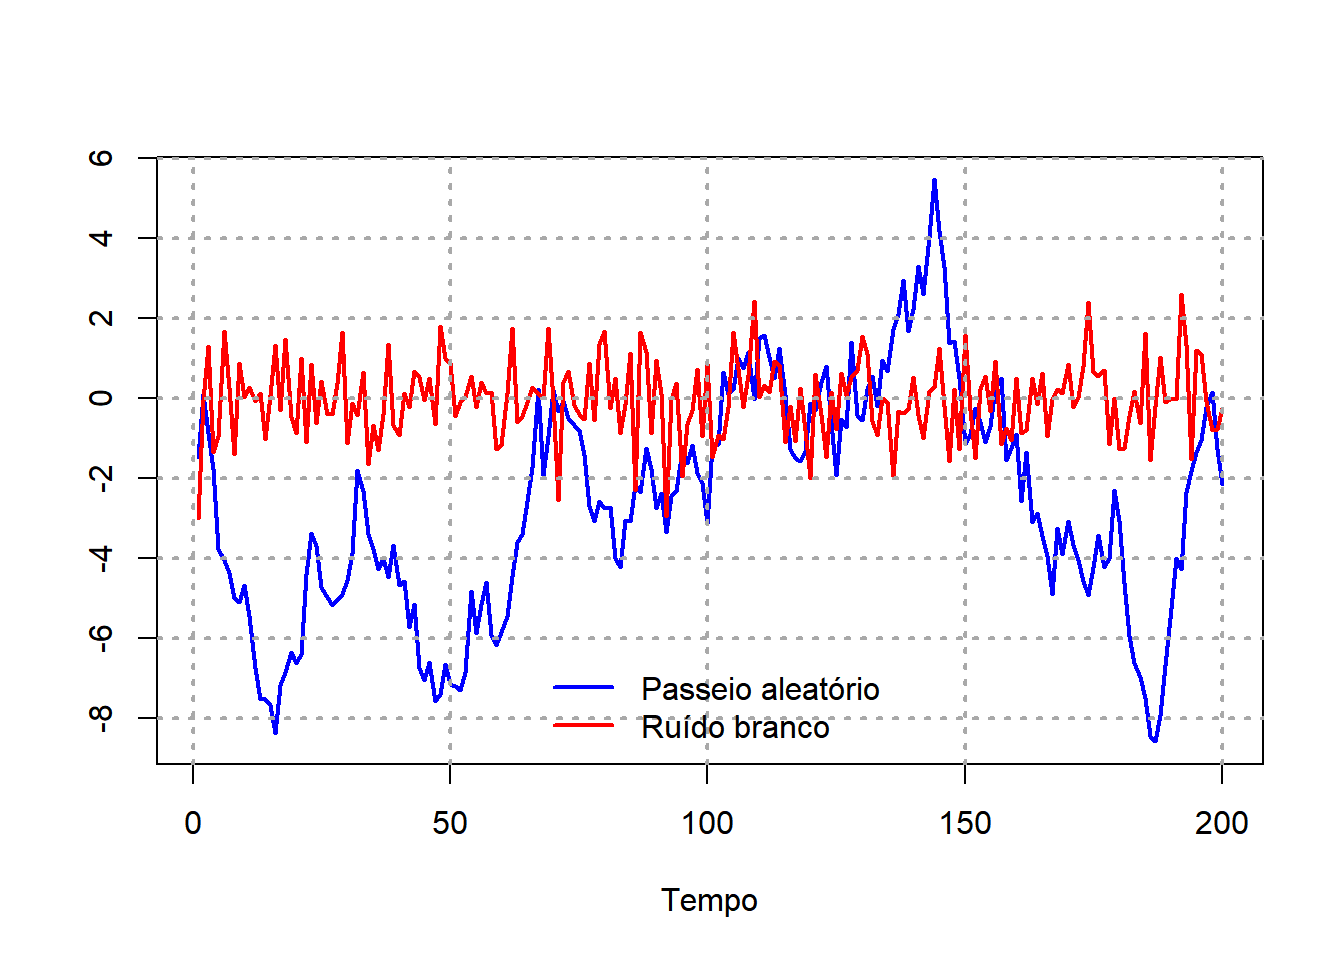
\includegraphics{Cap-2---Livro-de-Analise-de-Series-Temporais_files/figure-latex/unnamed-chunk-13-1.pdf}

\begin{Shaded}
\begin{Highlighting}[]
\KeywordTok{hist}\NormalTok{(FP, }\DataTypeTok{main =} \StringTok{"Distribuição da frequencia Folha de Pagamento"}\NormalTok{, }
     \DataTypeTok{xlab =} \StringTok{"Folha de Pagamento"}\NormalTok{,}\DataTypeTok{las=}\DecValTok{1}\NormalTok{ , }\DataTypeTok{col =} \StringTok{"373"}\NormalTok{)}
\end{Highlighting}
\end{Shaded}

\includegraphics{Cap-2---Livro-de-Analise-de-Series-Temporais_files/figure-latex/unnamed-chunk-13-2.pdf}

\begin{Shaded}
\begin{Highlighting}[]
\KeywordTok{hist}\NormalTok{(IC, }\DataTypeTok{main =} \StringTok{"Distribuição da frequencia indice de confiança"}\NormalTok{,}
     \DataTypeTok{xlab =} \StringTok{"Indice de confiança"}\NormalTok{,}\DataTypeTok{las=}\DecValTok{1}\NormalTok{ , }\DataTypeTok{col =} \StringTok{"373"}\NormalTok{)}
\end{Highlighting}
\end{Shaded}

\includegraphics{Cap-2---Livro-de-Analise-de-Series-Temporais_files/figure-latex/unnamed-chunk-13-3.pdf}

\begin{Shaded}
\begin{Highlighting}[]
\KeywordTok{hist}\NormalTok{(SC, }\DataTypeTok{main =} \StringTok{"Distribuição da frequencia Selic"}\NormalTok{, }
     \DataTypeTok{xlab =} \StringTok{"Selic"}\NormalTok{,}\DataTypeTok{las=}\DecValTok{1}\NormalTok{ , }\DataTypeTok{col =} \StringTok{"373"}\NormalTok{)}
\end{Highlighting}
\end{Shaded}

\includegraphics{Cap-2---Livro-de-Analise-de-Series-Temporais_files/figure-latex/unnamed-chunk-13-4.pdf}

\begin{Shaded}
\begin{Highlighting}[]
\KeywordTok{hist}\NormalTok{(TD, }\DataTypeTok{main =} \StringTok{"Distribuição da frequencia Taxa de Desemprego"}\NormalTok{, }
     \DataTypeTok{xlab =} \StringTok{"Taxa de Desemprego"}\NormalTok{,}\DataTypeTok{las=}\DecValTok{1}\NormalTok{ , }\DataTypeTok{col =} \StringTok{"373"}\NormalTok{)}
\end{Highlighting}
\end{Shaded}

\includegraphics{Cap-2---Livro-de-Analise-de-Series-Temporais_files/figure-latex/unnamed-chunk-13-5.pdf}

Boxplot

\#criando o gráfico

\begin{Shaded}
\begin{Highlighting}[]
\KeywordTok{boxplot}\NormalTok{(DE,}
         \DataTypeTok{xlab =} \StringTok{"Deposito em poupança"}\NormalTok{,}\DataTypeTok{las=}\DecValTok{1}\NormalTok{ , }\DataTypeTok{col =} \StringTok{"373"}\NormalTok{)}
\end{Highlighting}
\end{Shaded}

\includegraphics{Cap-2---Livro-de-Analise-de-Series-Temporais_files/figure-latex/unnamed-chunk-14-1.pdf}

\begin{Shaded}
\begin{Highlighting}[]
\KeywordTok{boxplot}\NormalTok{(FP,}
         \DataTypeTok{xlab =} \StringTok{"Folha de Pagamento"}\NormalTok{,}\DataTypeTok{las=}\DecValTok{1}\NormalTok{ , }\DataTypeTok{col =} \StringTok{"373"}\NormalTok{)}
\end{Highlighting}
\end{Shaded}

\includegraphics{Cap-2---Livro-de-Analise-de-Series-Temporais_files/figure-latex/unnamed-chunk-14-2.pdf}

\begin{Shaded}
\begin{Highlighting}[]
\KeywordTok{boxplot}\NormalTok{(IC,}
         \DataTypeTok{xlab =} \StringTok{"indice de confiança"}\NormalTok{,}\DataTypeTok{las=}\DecValTok{1}\NormalTok{ , }\DataTypeTok{col =} \StringTok{"373"}\NormalTok{)}
\end{Highlighting}
\end{Shaded}

\includegraphics{Cap-2---Livro-de-Analise-de-Series-Temporais_files/figure-latex/unnamed-chunk-14-3.pdf}

\begin{Shaded}
\begin{Highlighting}[]
\KeywordTok{boxplot}\NormalTok{(SC,}
         \DataTypeTok{xlab =} \StringTok{"Selic"}\NormalTok{,}\DataTypeTok{las=}\DecValTok{1}\NormalTok{ , }\DataTypeTok{col =} \StringTok{"373"}\NormalTok{)}
\end{Highlighting}
\end{Shaded}

\includegraphics{Cap-2---Livro-de-Analise-de-Series-Temporais_files/figure-latex/unnamed-chunk-14-4.pdf}

\begin{Shaded}
\begin{Highlighting}[]
\KeywordTok{boxplot}\NormalTok{(TD,}
         \DataTypeTok{xlab =} \StringTok{"Taxa de Desemprego"}\NormalTok{,}\DataTypeTok{las=}\DecValTok{1}\NormalTok{ , }\DataTypeTok{col =} \StringTok{"373"}\NormalTok{)}
\end{Highlighting}
\end{Shaded}

\includegraphics{Cap-2---Livro-de-Analise-de-Series-Temporais_files/figure-latex/unnamed-chunk-14-5.pdf}

Dispersão

\#criando o gráfico

\begin{Shaded}
\begin{Highlighting}[]
\KeywordTok{plot}\NormalTok{(DE, Ano,}
         \DataTypeTok{xlab =} \StringTok{"Deposito em poupança"}\NormalTok{, }\DataTypeTok{las=}\DecValTok{1}\NormalTok{, }\DataTypeTok{pch=}\DecValTok{19}\NormalTok{, }\DataTypeTok{col =} \StringTok{"black"}\NormalTok{)}
\end{Highlighting}
\end{Shaded}

\includegraphics{Cap-2---Livro-de-Analise-de-Series-Temporais_files/figure-latex/unnamed-chunk-15-1.pdf}

\begin{Shaded}
\begin{Highlighting}[]
\KeywordTok{plot}\NormalTok{(FP, Ano,}
         \DataTypeTok{xlab =} \StringTok{"Folha de Pagamento"}\NormalTok{, }\DataTypeTok{las=}\DecValTok{1}\NormalTok{, }\DataTypeTok{pch=}\DecValTok{19}\NormalTok{, }\DataTypeTok{col =} \StringTok{"black"}\NormalTok{)}
\end{Highlighting}
\end{Shaded}

\includegraphics{Cap-2---Livro-de-Analise-de-Series-Temporais_files/figure-latex/unnamed-chunk-15-2.pdf}

\begin{Shaded}
\begin{Highlighting}[]
\KeywordTok{plot}\NormalTok{(IC, Ano,}
         \DataTypeTok{xlab =} \StringTok{"indice de confiança"}\NormalTok{, }\DataTypeTok{las=}\DecValTok{1}\NormalTok{, }\DataTypeTok{pch=}\DecValTok{19}\NormalTok{, }\DataTypeTok{col =} \StringTok{"black"}\NormalTok{)}
\end{Highlighting}
\end{Shaded}

\includegraphics{Cap-2---Livro-de-Analise-de-Series-Temporais_files/figure-latex/unnamed-chunk-15-3.pdf}

\begin{Shaded}
\begin{Highlighting}[]
\KeywordTok{plot}\NormalTok{(SC, Ano,}
         \DataTypeTok{xlab =} \StringTok{"Selic"}\NormalTok{, }\DataTypeTok{las=}\DecValTok{1}\NormalTok{, }\DataTypeTok{pch=}\DecValTok{19}\NormalTok{, }\DataTypeTok{col =} \StringTok{"black"}\NormalTok{)}
\end{Highlighting}
\end{Shaded}

\includegraphics{Cap-2---Livro-de-Analise-de-Series-Temporais_files/figure-latex/unnamed-chunk-15-4.pdf}

\begin{Shaded}
\begin{Highlighting}[]
\KeywordTok{plot}\NormalTok{(TD, Ano,}
         \DataTypeTok{xlab =} \StringTok{"Taxa de Desemprego"}\NormalTok{, }\DataTypeTok{las=}\DecValTok{1}\NormalTok{, }\DataTypeTok{pch=}\DecValTok{19}\NormalTok{, }\DataTypeTok{col =} \StringTok{"black"}\NormalTok{)}
\end{Highlighting}
\end{Shaded}

\includegraphics{Cap-2---Livro-de-Analise-de-Series-Temporais_files/figure-latex/unnamed-chunk-15-5.pdf}

Gráfico de Barras

\#criando o gráfico

\begin{Shaded}
\begin{Highlighting}[]
\KeywordTok{barplot}\NormalTok{(DE, }\DataTypeTok{col =} \DecValTok{373}\NormalTok{)}
\end{Highlighting}
\end{Shaded}

\includegraphics{Cap-2---Livro-de-Analise-de-Series-Temporais_files/figure-latex/unnamed-chunk-16-1.pdf}

\begin{Shaded}
\begin{Highlighting}[]
\KeywordTok{barplot}\NormalTok{(FP, }\DataTypeTok{col =} \DecValTok{373}\NormalTok{)}
\end{Highlighting}
\end{Shaded}

\includegraphics{Cap-2---Livro-de-Analise-de-Series-Temporais_files/figure-latex/unnamed-chunk-16-2.pdf}

\begin{Shaded}
\begin{Highlighting}[]
\KeywordTok{barplot}\NormalTok{(IC, }\DataTypeTok{col =} \DecValTok{373}\NormalTok{)}
\end{Highlighting}
\end{Shaded}

\includegraphics{Cap-2---Livro-de-Analise-de-Series-Temporais_files/figure-latex/unnamed-chunk-16-3.pdf}

\begin{Shaded}
\begin{Highlighting}[]
\KeywordTok{barplot}\NormalTok{(SC, }\DataTypeTok{col =} \DecValTok{373}\NormalTok{)}
\end{Highlighting}
\end{Shaded}

\includegraphics{Cap-2---Livro-de-Analise-de-Series-Temporais_files/figure-latex/unnamed-chunk-16-4.pdf}

\begin{Shaded}
\begin{Highlighting}[]
\KeywordTok{barplot}\NormalTok{(TD, }\DataTypeTok{col =} \DecValTok{373}\NormalTok{)}
\end{Highlighting}
\end{Shaded}

\includegraphics{Cap-2---Livro-de-Analise-de-Series-Temporais_files/figure-latex/unnamed-chunk-16-5.pdf}

Ramos e Folhas

\#criando o gráfico

\begin{Shaded}
\begin{Highlighting}[]
\KeywordTok{stem}\NormalTok{(DE)}
\end{Highlighting}
\end{Shaded}

\begin{verbatim}
## 
##   The decimal point is 5 digit(s) to the right of the |
## 
##   0 | 
##   0 | 55555666666666666677777788888889999
##   1 | 00000000001111111111111111111111111111111112222222222233444444444444
##   1 | 55555566666666666667777777777889999
##   2 | 0001122334444
##   2 | 555666677788889
##   3 | 00012233344
##   3 | 556778889999
##   4 | 00111223334
##   4 | 567789
##   5 | 0011234
##   5 | 56788
##   6 | 00112234444444
##   6 | 5555555555555555566666666777889
##   7 | 001333344
##   7 | 567888
##   8 | 0
\end{verbatim}

\begin{Shaded}
\begin{Highlighting}[]
\KeywordTok{stem}\NormalTok{(FP)}
\end{Highlighting}
\end{Shaded}

\begin{verbatim}
## 
##   The decimal point is 1 digit(s) to the right of the |
## 
##    6 | 88
##    8 | 2355666666777899999900011222222233344445555566777888888888899
##   10 | 0001112245569999004688
##   12 | 0122334578891334455668
##   14 | 0056678134888
##   16 | 112248011567788888
##   18 | 00122222334458899111114555557
##   20 | 0002344455677788899901246678889999999999
##   22 | 01234468888888900012335578888888
##   24 | 00689004556677799
##   26 | 3444444668146
##   28 | 11111111994667
##   30 | 815
##   32 | 
##   34 | 
##   36 | 
##   38 | 2
##   40 | 
##   42 | 
##   44 | 
##   46 | 0
\end{verbatim}

\begin{Shaded}
\begin{Highlighting}[]
\KeywordTok{stem}\NormalTok{(IC)}
\end{Highlighting}
\end{Shaded}

\begin{verbatim}
## 
##   The decimal point is 1 digit(s) to the right of the |
## 
##    7 | 66789
##    8 | 14
##    8 | 556666777889999
##    9 | 0011111112223444444
##    9 | 555556667777888888889999999
##   10 | 00001111222222333334444444
##   10 | 555555666666777777778888888999999999
##   11 | 000001112222233333344444
##   11 | 5566667777799
##   12 | 01134444
##   12 | 5566788888899
##   13 | 00001112222233334444444
##   13 | 566777788889
##   14 | 000112233
##   14 | 5555566777899
##   15 | 233344
##   15 | 55566667778889
##   16 | 0000011111112233444
##   16 | 556
##   17 | 0
\end{verbatim}

\begin{Shaded}
\begin{Highlighting}[]
\KeywordTok{stem}\NormalTok{(SC)}
\end{Highlighting}
\end{Shaded}

\begin{verbatim}
## 
##   The decimal point is 1 digit(s) to the right of the |
## 
##   0 | 666666667777777777777788888888889999999999999
##   1 | 00000000000000000000011111111111111111111111111222222222222222223333+20
##   1 | 555555555556666666666666667777777777888888888888888899999999999
##   2 | 000000000111111111112222222222233344444
##   2 | 5555666667788
##   3 | 000022334
##   3 | 6779
##   4 | 12234
##   4 | 7889
##   5 | 
##   5 | 7
##   6 | 11
##   6 | 555
\end{verbatim}

\begin{Shaded}
\begin{Highlighting}[]
\KeywordTok{stem}\NormalTok{(TD)}
\end{Highlighting}
\end{Shaded}

\begin{verbatim}
## 
##   The decimal point is at the |
## 
##    6 | 9
##    7 | 4
##    7 | 5556678899999
##    8 | 00011112344
##    8 | 5555555667777778888899
##    9 | 0000000001111111111111222223333444444444
##    9 | 5556666667777788889999
##   10 | 000011112222223333333444444
##   10 | 55555555566667777777788888899999
##   11 | 00000111222233333334444
##   11 | 55555666667777778888889999
##   12 | 0000001223333444
##   12 | 55566677889999
##   13 | 12222233444
##   13 | 56699
##   14 | 01112223444
##   14 | 5556788
##   15 | 012
##   15 | 569
\end{verbatim}

Distribuição Empirica

\#criando o gráfico

\begin{Shaded}
\begin{Highlighting}[]
\NormalTok{nDE <-}\StringTok{ }\KeywordTok{length}\NormalTok{(DE)}
\NormalTok{yDE <-}\StringTok{ }\NormalTok{(}\DecValTok{1}\OperatorTok{:}\NormalTok{nDE)}\OperatorTok{/}\NormalTok{nDE}
\NormalTok{deDE <-}\StringTok{ }\KeywordTok{sort}\NormalTok{(DE)}
\KeywordTok{plot}\NormalTok{(DE, yDE, }\DataTypeTok{type =}\StringTok{"S"}\NormalTok{, }\DataTypeTok{xlab =}\StringTok{"Deposito em poupança"}\NormalTok{, }\DataTypeTok{ylab =}\StringTok{"Probabilidade"}\NormalTok{, }\DataTypeTok{main =}\StringTok{"Distribuição Empirica de Deposito em poupança"}\NormalTok{)}
\end{Highlighting}
\end{Shaded}

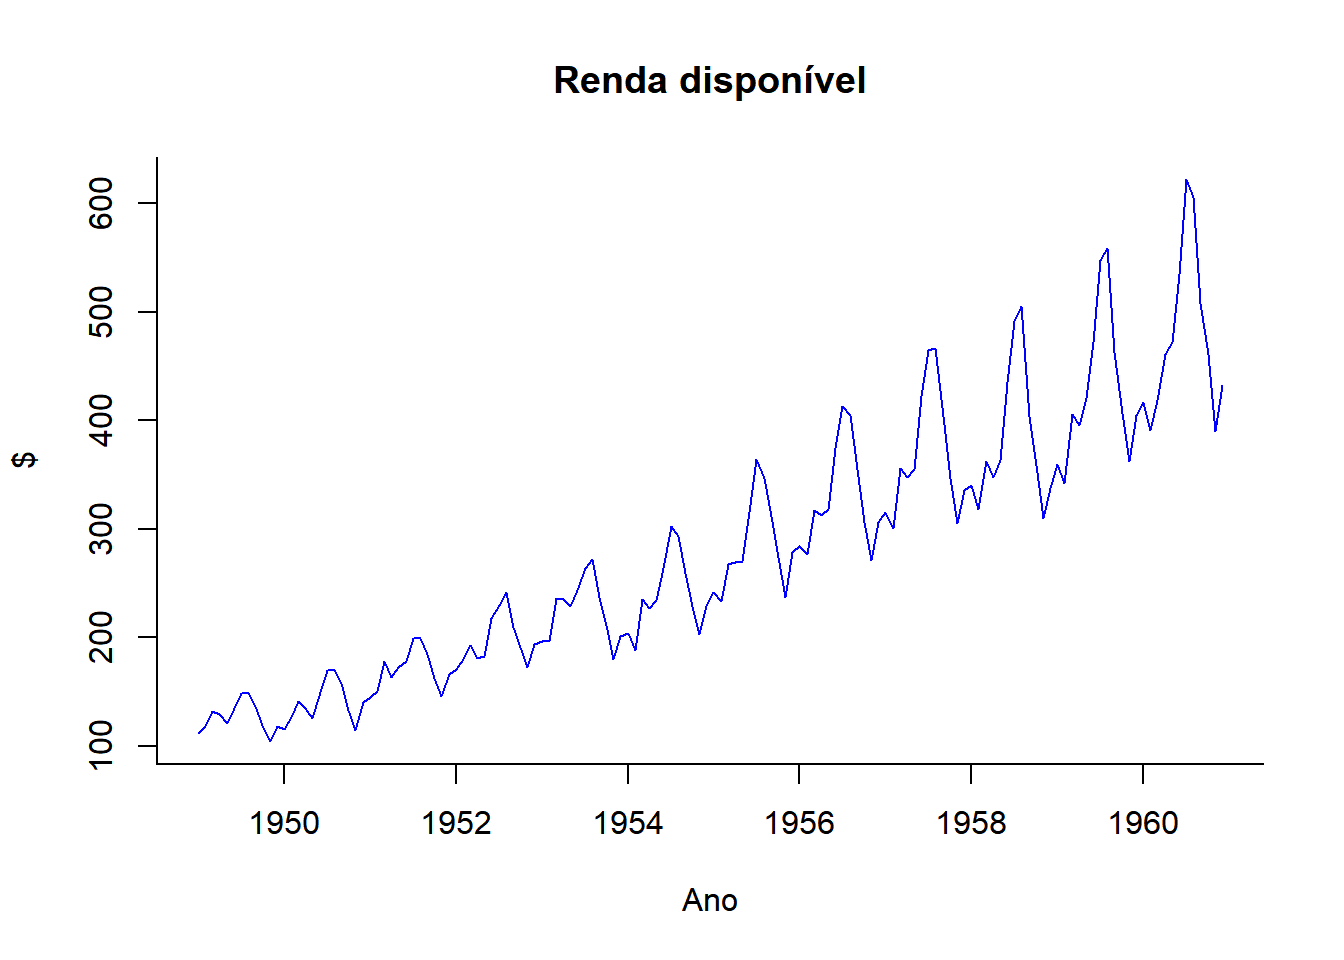
\includegraphics{Cap-2---Livro-de-Analise-de-Series-Temporais_files/figure-latex/unnamed-chunk-18-1.pdf}

\begin{Shaded}
\begin{Highlighting}[]
\NormalTok{nFP <-}\StringTok{ }\KeywordTok{length}\NormalTok{(FP)}
\NormalTok{yFP <-}\StringTok{ }\NormalTok{(}\DecValTok{1}\OperatorTok{:}\NormalTok{nFP)}\OperatorTok{/}\NormalTok{nFP}
\NormalTok{deFP <-}\StringTok{ }\KeywordTok{sort}\NormalTok{(FP)}
\KeywordTok{plot}\NormalTok{(FP, yFP, }\DataTypeTok{type =}\StringTok{"S"}\NormalTok{, }\DataTypeTok{xlab =}\StringTok{"Folha de Pagamento"}\NormalTok{, }\DataTypeTok{ylab =}\StringTok{"Probabilidade"}\NormalTok{, }\DataTypeTok{main =}\StringTok{"Distribuição Empirica de Folha de Pagamento"}\NormalTok{)}
\end{Highlighting}
\end{Shaded}

\includegraphics{Cap-2---Livro-de-Analise-de-Series-Temporais_files/figure-latex/unnamed-chunk-18-2.pdf}

\begin{Shaded}
\begin{Highlighting}[]
\NormalTok{nIC <-}\StringTok{ }\KeywordTok{length}\NormalTok{(IC)}
\NormalTok{yIC <-}\StringTok{ }\NormalTok{(}\DecValTok{1}\OperatorTok{:}\NormalTok{nIC)}\OperatorTok{/}\NormalTok{nIC}
\NormalTok{deIC <-}\StringTok{ }\KeywordTok{sort}\NormalTok{(IC)}
\KeywordTok{plot}\NormalTok{(IC, yIC, }\DataTypeTok{type =}\StringTok{"S"}\NormalTok{, }\DataTypeTok{xlab =}\StringTok{"indice de confiança"}\NormalTok{, }\DataTypeTok{ylab =}\StringTok{"Probabilidade"}\NormalTok{, }\DataTypeTok{main =}\StringTok{"Distribuição Empirica de indice de confiança"}\NormalTok{)}
\end{Highlighting}
\end{Shaded}

\includegraphics{Cap-2---Livro-de-Analise-de-Series-Temporais_files/figure-latex/unnamed-chunk-18-3.pdf}

\begin{Shaded}
\begin{Highlighting}[]
\NormalTok{nSC <-}\StringTok{ }\KeywordTok{length}\NormalTok{(SC)}
\NormalTok{ySC <-}\StringTok{ }\NormalTok{(}\DecValTok{1}\OperatorTok{:}\NormalTok{nSC)}\OperatorTok{/}\NormalTok{nSC}
\NormalTok{deSC <-}\StringTok{ }\KeywordTok{sort}\NormalTok{(SC)}
\KeywordTok{plot}\NormalTok{(SC, ySC, }\DataTypeTok{type =}\StringTok{"S"}\NormalTok{, }\DataTypeTok{xlab =}\StringTok{"Selic"}\NormalTok{, }\DataTypeTok{ylab =}\StringTok{"Probabilidade"}\NormalTok{, }\DataTypeTok{main =}\StringTok{"Distribuição Empirica Selic"}\NormalTok{)}
\end{Highlighting}
\end{Shaded}

\includegraphics{Cap-2---Livro-de-Analise-de-Series-Temporais_files/figure-latex/unnamed-chunk-18-4.pdf}

\begin{Shaded}
\begin{Highlighting}[]
\NormalTok{nTD <-}\StringTok{ }\KeywordTok{length}\NormalTok{(TD)}
\NormalTok{yTD <-}\StringTok{ }\NormalTok{(}\DecValTok{1}\OperatorTok{:}\NormalTok{TD)}\OperatorTok{/}\NormalTok{TD}
\NormalTok{deTD <-}\StringTok{ }\KeywordTok{sort}\NormalTok{(TD)}
\KeywordTok{plot}\NormalTok{(TD, yTD, }\DataTypeTok{type =}\StringTok{"S"}\NormalTok{, }\DataTypeTok{xlab =}\StringTok{"Taxa de Desemprego"}\NormalTok{, }\DataTypeTok{ylab =}\StringTok{"Probabilidade"}\NormalTok{, }\DataTypeTok{main =}\StringTok{"Distribuição Empirica de Taxa de Desemprego"}\NormalTok{)}
\end{Highlighting}
\end{Shaded}

\includegraphics{Cap-2---Livro-de-Analise-de-Series-Temporais_files/figure-latex/unnamed-chunk-18-5.pdf}


\end{document}
